% 鈴木研究室 卒業論文テンプレート
% Version: 1.8
% Last Update: 2016/12/22 by Hidekazu Suzuki
% Contact to: hsuzuki@meijo-u.ac.jp
% Character code: UTF-8

% TexStudio もしくは Texmaker のオプション>設定>コマンド>LaTexの項目をよく確認して下記 documentclass を適宜選択
%platexを用いてコンパイルする場合(2015年度以前にLaTex環境を構築した人はこっち)
%\documentclass[a4j,11pt]{jreport}
%uplatexを用いてコンパイルする場合(2016年度以降,Tex LiveでLaTex環境を構築した人はこっち)
\documentclass[a4j,11pt]{ujreport}
\usepackage{UCLabThesis}

%--------------------------------------------------------------
% 表紙
%--------------------------------------------------------------

% 論文種類(変更しないこと!!)
\bachelor		% 卒業論文
%\master	% 修士論文
%\thesis		% 博士論文

% 卒業年度
\gyear{平成23}

% タイトル(和文・英文)
% 長い場合は自動的に改行される.「\\」の挿入で任意の位置で改行可能.
\title{鈴木研究室における卒業論文テンプレートの\\使い方に関する研究}
\etitle{A Study on How to Use Template of\\Bachelor Thesis in Suzuki Laboratory}

% 著者(姓と名の間に全角スペース)
\author{鈴木 秀和}

% 学籍番号
\studentid{080427000}

% 論文提出日
\date{平成24年2月10日}

\begin{document}
% 表紙(消さないこと!!)
\maketitle
% 表紙裏を白紙にする(消さないこと!!)
\cleardoublepage

%--------------------------------------------------------------
% アブストラクト
%--------------------------------------------------------------
% 和文
\begin{abstract}
ここに卒業研究の概要を和文で記述する.
\end{abstract}
% 英文
\begin{eabstract}
You must write an abstract of your bachelor thesis in English here.
\end{eabstract}
\cleardoublepage

% 目次(消さないこと!!)
\tableofcontents
\cleardoublepage


%--------------------------------------------------------------
% ここから本文
%--------------------------------------------------------------

% ページ番号をアラビア数字に変更(消さないこと!!)
\pagenumbering{arabic}

%---序論(ここから)------------------------------------------
\chapter{序論}\label{chap:Intro}

鈴木研究室では,{\LaTeX}により卒業論文を執筆することとしている.
{\LaTeX}を用いることにより,簡単に卒業論文の体裁に則った出力が得られるため,体裁に関する不備を最小限に抑えることができ,文章を記述することに専念できる.
また,鈴木研究室では日常の研究報告資料や学会発表論文を{\LaTeX}で作成しているため,それらの資産を活用することにより,効率よく論文を執筆することも可能である.

この文章\footnote{\texttt{bthesis.tex}}は卒業論文のスタイルファイル\footnote{\texttt{UCLabThesis.sty}}を利用して作成されているため,各自が卒業論文を執筆する場合にテンプレートとして参考・使用されたい.
なお,この{\TeX}ファイルおよび鈴木研究室用スタイルファイルはUTF-8で作成されているため,特にWindows PCにおいて編集時にShift JISなどの別の文字コードに変更しないよう注意してほしい.

%---序論(ここまで)------------------------------------------

%---スタイルファイルの使い方(ここから)--------------------------------------
\chapter{スタイルファイルの使い方}\label{chap:HowTo}

\section{構成}
\label{sec:Structure}

卒業論文は下記の要素から構成しなければならない.

\subsection{表紙}
\label{subsec:TitlePage}
卒業論文の表紙には,下記コマンドにより対応する情報を記載する.

\begin{itemize}
\item \cmd{bachelor}:\mbox{}\\
卒業論文用タイトルページのフォーマットにする.
修士論文または博士論文の場合はこの記述をコメントアウトし,それぞれ\cmd{master}または\cmd{thesis}を指定する.

\item \cmd{gyear}:\mbox{}\\
\verb|\gyear{平成23}|のように,卒業年度を和暦(元号+年度)で入力する.

\item \cmd{title},\cmd{etitle}:\mbox{}\\
卒業論文の題目を和文,英文で入力する.
題目が長い場合は自動的に改行されるが,文節などの区切り箇所に適宜``\verb|\\|''を挿入・改行した方が見栄えが良くなる.

\item \cmd{author}:\mbox{}\\
著者名を記述する.
ここで言う著者とは,卒業論文を執筆する本人1名のみである.
なお,記述する際には\verb|\author{鈴木 秀和}|のように姓と名の間に全角スペースを1文字入力すること.

\item \cmd{studentid}:\mbox{}\\
学籍番号を省略せずに入力する.

\item \cmd{date}:\mbox{}\\
\verb|\date{平成24年2月10日}|のように,卒業論文提出日を和暦(元号+年月日)で入力する.
\end{itemize}

\begin{boxnote}
なお,学科事務室へ卒業論文を提出する際は,情報工学科ローカルサーバ\url{http://rjie.meijo-u.ac.jp/}の「卒業論文」ページに用意されている専用タイトルページ(Word形式)に差し替えること.
\end{boxnote}

\subsection{概要}
卒業論文の概要は,\cmd{abstract}環境と\cmd{eabstract}環境により,それぞれ和文と英文で記述する.

\begin{code}
\begin{abstract}
和文アブストラクト
\end{abstract}

\begin{eabstract}
English abstract
\end{eabstract}
\end{code}%

\subsection{目次}
目次は\cmd{tableofcontents}\footnote{「概要」の後に記述されている.絶対に消さないこと.}の記載があれば,{\LaTeX}のコンパイルにより自動的に生成される.

\subsection{論文本体}
ここから論文の本体(「第1章」から「まとめ」まで)を記述する.
分量が多くなり1つの{\TeX}ファイルでの管理が大変になった場合は,\cmd{input}コマンドを用いて外部{\TeX}ファイルを読み込む形式にするとよい.
なお,\pageref{chap:Achievement}ページ以降の研究業績および付録は,それぞれ\texttt{achievement.tex}および\texttt{appendix.tex}を読み込んでいる.

この{\TeX}ファイルは\texttt{jreport}スタイルを採用しているため,\tabref{tab:HeadCommands}に示すコマンドを使用して章節項を設定する.

\begin{table}[ht]
	\centering
	\caption{章節項目を設定するコマンド一覧}
	\label{tab:HeadCommands}
	\small
	\begin{tabular}{l|l}
		\Hline 
		コマンド & 説明 \\ 
		\hline\hline
		\cmd{chapter} & 章を設定するコマンド.章番号が割り当てられる.(例:\chapref{chap:HowTo})\\ 
		\cmd{section} & 節を設定するコマンド.節番号が割り当てられる.(例:\secref{sec:Structure})\\ 
		\cmd{subsection} & 項を設定するコマンド.項番号が割り当てられる.(例:\subsecref{subsec:TitlePage})\\ 
		\cmd{subsubsection} & 目を設定するコマンド.ただし目番号は割り当てられない.\\ 
		\hline 
	\end{tabular} 
\end{table}

\subsection{謝辞}
研究を遂行するに当たり,お世話になった教員,研究者,学生らに対する謝辞を,\texttt{gratitude}環境を用いて記述する.

\begin{code}
\begin{gratitude}
ここに謝辞を記述する.
\end{gratitude}
\end{code}%

\subsection{参考文献}
参考文献リストを掲載する.
詳細は\secref{sec:reference}を参照.

\subsection{研究業績}
研究活動における研究業績を掲載する.
詳細は\secref{sec:achievement}を参照.

\subsection{付録}
論文本体には記述する必要はないが,補足資料として掲載する場合は付録として\cmd{appendix}の記載以降に記述する.
章節などのコマンドは,論文本体と同様に利用することができる.
付録については,\pageref{apdx:Example}ページを参照.

\section{ラベルの命名規則と独自参照コマンド}

\subsection{ラベルの命名規則}
章・節・項や図表などの項目に,\cmd{label}を用いてラベルを設定することにより,本文中から適切に参照することができる.
このとき,ラベルフォーマットを\tabref{tab:NamingConventions}の規則に則って記述すれば,ラベル名を見るだけである程度の項目種別が類推できる.
なお,本文章のラベルもこの命名規則に則って設定しているので参照されたい.

\subsection{独自参照コマンド}
{\LaTeX}では通常,章節や図表の参照に以下のように\cmd{ref}を用いるが,毎回「$\bigcirc$章」,「$\bigcirc$節」,「図$\bigcirc$」,「表$\bigcirc$」のように文字を記入するのは面倒である.
そこで,本テンプレートでは各項目の参照には下記のような独自のコマンドを定義している.
本文中で参照を利用する場合は,\tabref{tab:ReferenceCommands}に示すコマンドを利用する.

\begin{table}[b]
	\centering
	\begin{tabular}{c}
		% 左側の表
		\begin{minipage}[t]{0.33\hsize}
			\centering
			\caption{ラベルの命名規則}
			\label{tab:NamingConventions}
			\small
			\begin{tabular}{l|l}
				\Hline 
				項目 & ラベルフォーマット \\ 
				\hline\hline
				章 & \texttt{chap:LABEL} \\ 
				節 & \texttt{sec:LABEL} \\ 
				項 & \texttt{subsec:LABEL} \\ 
				付録 & \texttt{apdx:LABEL} \\ 
				図 & \texttt{fig:LABEL} \\ 
				表 & \texttt{tab:LABEL} \\ 
				数式 & \texttt{eq:LABEL} \\ 
				\hline 
			\end{tabular} 
		\end{minipage}%
		% 右側の表
		\begin{minipage}[t]{0.66\hsize}
			\centering
			\caption{独自参照コマンド一覧}
			\label{tab:ReferenceCommands}
			\small
			\begin{tabular}{l|l}
				\Hline 
				コマンド & 説明 \\ 
				\hline\hline
				\cmd{chapref} & \cmd{chapter}で設定された章を参照\\
				\cmd{secref} & \cmd{section}で設定された節を参照\\
				\cmd{subsecref} & \cmd{subsection}で設定された項を参照\\
				\cmd{apdxref} & 付録の各章・節・項を参照\\
				\cmd{figref} & 図を参照\\
				\cmd{tabref} & 表を参照\\
				\cmd{eqref} & 数式を参照\\
				\hline 
			\end{tabular} 
		\end{minipage}
	\end{tabular}
\end{table}


\section{図表}

\subsection{図}
図は拡大縮小しても美しく表示されるように,できる限りベクタ図で作成することが望ましい.
ベクタ図はPowerPointやVisioなどで作図し,EPSファイルに変換して生成することができる.
EPSファイルの変換方法は,鈴木研究室Wikiページ\footnote{\url{https://sites.google.com/a/ccalumni.meijo-u.ac.jp/uclab-wiki/latex/figure}}を参照すること.
ラスタ図はスクリーンキャプチャや写真などの図に限定し,PNGファイルやJPEGファイルとして用意する.

ただし,JPEGファイルなど画像ファイルのままでは貼り付けられない.
コマンドプロンプトを開き,\verb|extractbb|コマンドを用いて.xbbファイルを生成しておく必要がある.

コマンド例:\verb|extractbb logo.png|

\texttt{figure}環境を用いて下記のテンプレートに従って図を掲載する.
\texttt{figure}環境の位置オプションには\tabref{tab:FigureOptions}に示すものが利用でき,図の挿入位置を指定することができる.
このオプションは複数指定できるが,先頭に書いたオプションが優先される.
\cmd{includegraphics}コマンドのオプションには\tabref{tab:IncludegraphicsOptions}に示すものが利用でき,コンマ区切りで複数指定できる.

\begin{code}
\begin{figure}[位置]
	\centering
	\includegraphics[オプション]{画像ファイルの相対パス}
	\caption{キャプション}
	\label{fig:ラベル}
\end{figure}
\end{code}%

\begin{figure}[ht]
	\centering
	
\includegraphics[clip,scale=0.3]{fig/tiger.eps}
	\caption{EPSファイルの読み込み}
	\label{fig:ExampleEPS}
\end{figure}

\begin{figure}[ht]
	\centering
	
\includegraphics[autoebb,clip,height=3.0cm]{fig/logo.png}
	\caption{PNGファイルの読み込み}
	\label{fig:ExamplePNG}
\end{figure}

\begin{table}[ht]
	\centering
	\caption{\texttt{figure}環境で指定できる挿入位置}
	\label{tab:FigureOptions}
	\small
	\begin{tabular}{l|l}
		\Hline 
		オプション & 説明 \\ 
		\hline\hline
		\texttt{h} & 図を\texttt{figure}環境を記述した位置に挿入\\
		\texttt{t} & 図をページの上部に挿入\\
		\texttt{b} & 図をページの下部に挿入\\
		\hline 
	\end{tabular} 
\end{table}

\begin{table}[ht]
	\centering
	\caption{\cmd{includegraphics}コマンドのオプション一覧}
	\label{tab:IncludegraphicsOptions}
	\small
	\begin{tabular}{l|l}
		\Hline 
		オプション & 説明 \\ 
		\hline\hline
		\texttt{width=}$SIZE$ & 図の幅を$SIZE$で指定(例:\texttt{width=5.5cm})\\
		\texttt{height=}$SIZE$ & 図の高さを$SIZE$で指定(例:\texttt{height=4.0cm})\\
		\texttt{scale=}$RATIO$ & 図の大きさを$RATIO$で指定した比率で拡大縮小(例:\texttt{scale=0.8})\\
		\texttt{clip} & 描画領域(Bounding Box)のみを出力.とりあえず設定しておけばよい.\\
		\texttt{autoebb} & PNGやJPEGを読み込む場合は,必ず指定する.\\
		\hline 
	\end{tabular} 
\end{table}

\subsection{表}

\texttt{table}環境を用いて下記のテンプレートに従って表を作成する.
\texttt{table}環境の位置オプションには図と同様に\tabref{tab:FigureOptions}に示すものが利用でき,表の挿入位置を指定することができる.

\begin{code}
\begin{table}[位置]
	\centering 
	\caption{キャプション}
	\label{tab:ラベル}
	\small	% 表中の文字サイズを指定
	\begin{tabular}{l|ll}
		\Hline 
		列見出し0 & 列見出し1 & 列見出し2\\ 
		\hline\hline
		行見出し1 & データ11 & データ12\\
		行見出し2 & データ21 & データ22\\
		\hline 
	\end{tabular} 
\end{table}
\end{code}%

表を作成する際には,以下のポイントをおさえておくとよい.
\begin{itemize}
\item セルの行揃えはデータが文字列の場合は左揃え,数値の場合は右揃えとする.
中央揃えは$\bigcirc$や$\times$などの記号を表記する場合に限定した方が見やすい.
\item キャプション下の罫線(表の最上部の罫線)は\cmd{Hline}により太線にする.
\item 列見出しとデータ領域の間は\cmd{hline}を2つ記述して二重線にする.
\item データエリアは見やすさを考慮して,できる限り罫線は引かない.
\item 表の最下部の罫線は必ず引く.
\item 表中の文字サイズを小さくしたい場合は,\cmd{centering}の後ろに\cmd{small}などの文字サイズを指定するコマンドを入力する.
\end{itemize}

\begin{table}[ht]
	\centering
	\caption{テンプレートに示した表の作成例}
	\label{tab:ExampleTable}
	\small
	\begin{tabular}{l|ll}
		\Hline 
		列見出し0 & 列見出し1 & 列見出し2\\ 
		\hline\hline
		行見出し1 & データ11 & データ12\\
		行見出し2 & データ21 & データ22\\
		\hline 
	\end{tabular} 
\end{table}

\subsection{並列配置}
スペースの有効活用のために図表を並べて掲載したい場合,キャプションをどのように設定するかにより,次の2種類の方法がある.

\subsubsection{\underline{個別のキャプションを設定する場合}}
図を並べて掲載する場合は,\texttt{figure}環境内に\texttt{minipage}環境を用いて指定した幅のページを作成し,その中に図を読み込む.

\begin{code}
\begin{figure}[位置オプション1]
	\centering
	% 左側の図
	\begin{minipage}[位置オプション2]{幅}
		\centering
		\includegraphics[〜]{〜}
		\caption{〜}
		\label{〜}
	\end{minipage}% ←この%は削除しないこと
	% 右側の図
	\begin{minipage}[位置オプション2]{幅}
		2番目の図(省略)
	\end{minipage}
\end{figure}
\end{code}%

\begin{description}
\item[位置オプション1(\texttt{figure}環境):]\mbox{}\\
並列で掲載した図表を1つの組として考え,その掲載位置を指定する.
位置の指定は前述した図表と同様で,\tabref{tab:FigureOptions}に示すオプションのいずれかを指定する.

\item[位置オプション2(\texttt{minipage}環境):]\mbox{}\\
各図表の上下位置を指定する.
位置指定には下記に示す通り,並列で掲載する内容に応じて指定する.
\begin{itemize}
\item 2つとも図の場合:\texttt{[b]}を指定して,図のキャプション位置を揃える.
\item 2つとも表の場合:\texttt{[t]}を指定して,表のキャプション位置を揃える.
\item 図と表1つずつの場合:\texttt{[\,]}のように何も指定しなくてもよい.
\end{itemize}

\item[幅:]\mbox{}\\
ページの幅を指定する.
\texttt{10cm}のように固定値で設定することもできるが,通常は下記のようにページ幅(\cmd{hsize}で取得)を掲載する図表の数に分割する.
\begin{itemize}
\item 2つ並べて掲載する場合:\texttt{0.5}\cmd{hsize}
\item 3つ並べて掲載する場合:\texttt{0.33}\cmd{hsize}
\end{itemize}
\end{description}

\begin{figure}[ht]
	\centering
	% 左側の図
	\begin{minipage}[b]{0.5\hsize}
		\centering
		
\includegraphics[clip,height=5.0cm]{fig/tiger.eps}
		\caption{図の並列掲載例(左側)}
		\label{fig:ExampleParallelFigureLeft}
	\end{minipage}% ←この%は削除しないこと
	% 右側の図
	\begin{minipage}[b]{0.5\hsize}
		\centering
		
\includegraphics[clip,height=3.0cm]{fig/tiger.eps}
		\caption{図の並列掲載例(右側)}
		\label{fig:ExampleParallelFigureRight}
	\end{minipage}
\end{figure}

表を並べて掲載する場合は,\texttt{table},\texttt{tabular}環境内に\texttt{minipage}環境を用いて指定した幅のページを作成し,その中に表を作成する.

\begin{code}
\begin{table}[位置オプション1]
	\centering
	\begin{tabular}{c}
		% 左側の表
		\begin{minipage}[位置オプション2]{幅}
			\centering 
			\caption{〜}
			\label{〜}
			\small
			\begin{tabular}{〜}
				\Hline 
				〜\\ 
				\hline\hline
				〜\\
				\hline 
			\end{tabular} 
		\end{minipage}% ←この%は削除しないこと
		% 右側の表
		\begin{minipage}[位置オプション2]{幅}
			2番目の表(省略)
		\end{minipage}
	\end{tabular}
\end{table}
\end{code}%

\begin{table}[ht]
	\centering
	\begin{tabular}{c}
		% 左側の表
		\begin{minipage}[t]{0.5\hsize}
			\centering 
			\caption{表の並列掲載例(左側)}
			\label{tab:ExampleParallelTableLeft}
			\small
			\begin{tabular}{l|ll}
				\Hline 
				列見出し0 & 列見出し1 & 列見出し2\\ 
				\hline\hline
				行見出し1 & データ11 & データ12\\
				行見出し2 & データ21 & データ22\\
				行見出し3 & データ31 & データ32\\
				\hline 
			\end{tabular} 
		\end{minipage}% ←この%は削除しないこと
		% 右側の表
		\begin{minipage}[t]{0.5\hsize}
			\centering 
			\caption{表の並列掲載例(右側)}
			\label{tab:ExampleParallelTableRight}
			\small
			\begin{tabular}{l|ll}
				\Hline 
				列見出し0 & 列見出し1 & 列見出し2\\ 
				\hline\hline
				行見出し1 & データ11 & データ12\\
				行見出し2 & データ21 & データ22\\
				行見出し3 & データ31 & データ32\\
				行見出し4 & データ41 & データ42\\
				行見出し5 & データ51 & データ52\\
				\hline 
			\end{tabular} 
		\end{minipage}
	\end{tabular}
\end{table}

図と表を並べて掲載する場合は,\texttt{figure}環境内または\texttt{table}環境内のどちらかに\texttt{minipage}環境を用いて指定した幅のページを作成し,その中に図を読み込みと,表の作成を行えばよい.
ただし,キャプションの設定には次の点を注意する必要がある.

\begin{description}
\item[\texttt{figure}環境を用いる場合:]\mbox{}\\
図のキャプションは\cmd{caption}で指定すればよいが,表のキャプションは\cmd{caption}で指定してしまうと「表」ではなく「図」と表記してしまう.
そのため,表のキャプションには独自定義した\cmd{tabcaption}コマンドを用いて設定する.

\begin{figure}[ht]
	\centering
	\begin{tabular}{c}
		% 左側の図
		\begin{minipage}[]{0.5\hsize}
			\centering 
			
\includegraphics[clip,height=4.0cm]{fig/tiger.eps}
			\caption{図表の並列掲載例1(左側を図とした場合)}
			\label{fig:ExampleParallelMixLeft1}
		\end{minipage}% ←この%は削除しないこと
		% 右側の表
		\begin{minipage}[]{0.5\hsize}
			\centering
			\tabcaption{図表の並列掲載例1(右側を表とした場合)}
			\label{tab:ExampleParallelMixRight1}
			\small
			\begin{tabular}{l|ll}
				\Hline 
				列見出し0 & 列見出し1 & 列見出し2\\ 
				\hline\hline
				行見出し1 & データ11 & データ12\\
				行見出し2 & データ21 & データ22\\
				行見出し3 & データ31 & データ32\\
				\hline 
			\end{tabular}
		\end{minipage}
	\end{tabular}
\end{figure}

\item[\texttt{table}環境を用いる場合:]\mbox{}\\
表のキャプションは\cmd{caption}で指定すればよいが,図のキャプションは\cmd{caption}で指定してしまうと「図」ではなく「表」と表記してしまう.
そのため,図のキャプションには独自定義した\cmd{figcaption}コマンドを用いて設定する.

\begin{table}[ht]
	\centering
	% 左側の表
	\begin{minipage}[]{0.5\hsize}
		\centering 
		\caption{図表の並列掲載例2(左側を表とした場合)}
		\label{tab:ExampleParallelMixLeft2}
		\small
		\begin{tabular}{l|ll}
			\Hline 
			列見出し0 & 列見出し1 & 列見出し2\\ 
			\hline\hline
			行見出し1 & データ11 & データ12\\
			行見出し2 & データ21 & データ22\\
			行見出し3 & データ31 & データ32\\
			\hline 
		\end{tabular}
	\end{minipage}% ←この%は削除しないこと
	% 右側の図
	\begin{minipage}[]{0.5\hsize}
		\centering
		
\includegraphics[clip,height=4.0cm]{fig/tiger.eps}
		\figcaption{図表の並列掲載例2(右側を図とした場合)}
		\label{fig:ExampleParallelMixRight2}
	\end{minipage}
\end{table}

\end{description}

\subsubsection{\underline{サブキャプションを設定する場合}}
図を並列で記載するがキャプションは1つにしたい場合は\texttt{subfig}環境を利用して実現する.
\texttt{subfig}環境を利用する場合は,各図にサブキャプションを設定することができる.
また,各図にラベルを設定できるが,図全体しか参照しない場合は設定する必要はない(\cmd{subfloat}内の\cmd{label}).
図の参照は\cmd{figref}コマンドを用いれば,通常の図と同じように\figref{fig:ExampleSubfig}の他,\figref{fig:ExampleSubfigFigure1}や\figref{fig:ExampleSubfigFigure2}のように個々の図を参照することもできる.

\begin{figure}[ht]
	\centering
	\subfloat[1匹目のタイガー]{%
		
\includegraphics[clip,height=3.0cm]{fig/tiger.eps}
		\label{fig:ExampleSubfigFigure1}
	}%
	\qquad
	\subfloat[2匹目のタイガー]{%
		
\includegraphics[clip,height=3.0cm]{fig/tiger.eps}
		\label{fig:ExampleSubfigFigure2}
	}%
	\qquad
	\subfloat[3匹目のタイガー]{%
		
\includegraphics[clip,height=3.0cm]{fig/tiger.eps}
		\label{fig:ExampleSubfigFigure3}
	}%
	\caption{\texttt{subfig}環境を用いた図の並列表記例}
	\label{fig:ExampleSubfig}
\end{figure}

\begin{code}
\begin{figure}[位置オプション]
	\centering
	% 1つ目の図
	\subfloat[サブキャプション1]{%
		\includegraphics[〜]{〜}
		\label{1つ目の図のラベル}
	}%
	\qquad % 2つの図の間の空白
	% 2つ目の図
	\subfloat[サブキャプション2]{%
		\includegraphics[〜]{〜}
		\label{2つ目の図のラベル}
	}%
	\caption{図全体のキャプション}
	\label{図全体のラベル}
\end{figure}
\end{code}


\section{箇条書き}

{\LaTeX}の箇条書き用の環境である\cmd{enumerate}, \cmd{itemize}, \cmd{description}を,状況に応じて使い分ければよい.
ただし,本スタイルファイル\texttt{UCLabThesis.sty}を採用している場合は,通常の箇条書き環境と比較してリストの間隔が狭く,通常の行間隔と同じ設定になっている.

\subsection{itemize}
\texttt{itemize}環境を用いれば,記号付き箇条書きを記述できる.
箇条書きの記号は1段目から順に「$\bullet$」,「--」,「$\ast$」となる.

\begin{screen}
\begin{itemize}
\renewcommand{\labelitemi}{#}
\item 項目1
\item 項目2
\begin{itemize}
\item 項目2-1
\begin{itemize}
\item 項目2-1-1
\end{itemize}
\end{itemize}
\item 項目3
\end{itemize}
\end{screen}

記号はできる限り標準のものを使用することが望ましいが,変更したい場合は下記のように\cmd{renewcommand}により\cmd{labelitemi}の記号を指定したものに変更できる.

\begin{minipage}[t]{0.7\hsize}
\begin{code}
\begin{itemize}
\renewcommand{\labelitemi}{■}
\item 項目1
\end{code}
\end{minipage}
\quad
\begin{minipage}[t]{0.25\hsize}
\begin{screen}
\begin{itemize}
\renewcommand{\labelitemi}{■}
\item 項目1
\item 項目2
\end{itemize}
\end{screen}
\end{minipage}

\subsection{enumerate}
\texttt{enumerate}環境を用いれば,番号付き箇条書きを記述できる.
箇条書きの表記は1段目から順に「(\,1\,)」,「(\,a\,)」,「i.」となる.

\begin{screen}
\begin{enumerate}
\item 項目1
\item 項目2
\begin{enumerate}
\item 項目2-1
\begin{enumerate}
\item 項目2-1-1
\end{enumerate}
\end{enumerate}
\item 項目3
\end{enumerate}
\end{screen}

\verb|\begin{enumerate}|の直後にオプションを指定することにより,番号付き箇条書きの表記を変更することができる.
番号部分を変更する場合は,``\texttt{label=}''で表記を設定する.
詳細は{\TeX}文章または\texttt{enumitem.sty}の解説ページ
\footnote{例えば,\url{http://xyoshiki.web.fc2.com/tex/enumitem.html}が参考になる.}
を参照されたい.

\begin{minipage}[t]{0.7\hsize}
\begin{code}
% \Alphは大文字のアルファベットを意味する
\begin{enumerate}[label=\Alph*\,)]
\item 〜
\end{code}
\end{minipage}
\quad
\begin{minipage}[t]{0.25\hsize}
\begin{screen}
% \Alphは大文字のアルファベットを意味する
\begin{enumerate}[label=\Alph*\,)]
\item 項目1
\item 項目2
\item 項目3
\end{enumerate}
\end{screen}
\end{minipage}

\begin{minipage}[t]{0.7\hsize}
\begin{code}
% \Romanは大文字のローマ数字を意味する
\begin{enumerate}[label=\Roman*.]
\item 〜
\end{code}
\end{minipage}
\quad
\begin{minipage}[t]{0.25\hsize}
\begin{screen}
% \Romanは大文字のローマ数字を意味する
\begin{enumerate}[label=\Roman*.]
\item 項目1
\item 項目2
\item 項目3
\end{enumerate}
\end{screen}
\end{minipage}

また,\cmd{label}コマンドにより項目にラベルを設定することにより,\cmd{ref}コマンドを用いて\ref{item:Step1},\ref{item:Step2}のように参照することもできる.

\begin{code}
% \arabicは小文字のアラビア数字,font=\bfseriesは太字を意味する
\begin{enumerate}[label=Step \arabic*.,leftmargin=*,font=\bfseries]
\item 〜
\end{code}

\begin{screen}
% \arabicは小文字のアラビア数字,font=\bfseriesは太字を意味する
\begin{enumerate}[label=Step \arabic*.,leftmargin=*,font=\bfseries]
\item 項目1
\label{item:Step1}
\item 項目2
\label{item:Step2}
\item 項目3
\label{item:Step3}
\end{enumerate}
\end{screen}

\subsection{description}
\texttt{description}環境を用いれば,見出し付き箇条書きを記述できる.
見出しは\verb|\item[項目1]|のように``\texttt{[\,]}''内に記述し,太字で表記される.

\begin{screen}
\begin{description}
\item[項目1]あいうえお
\item[項目2]かきくけこ
\item[項目3]さしすせそ
\end{description}
\end{screen}

見出しの後に改行する場合は,見出しの直後に\verb|\mbox{}\\|を入力して改行する.

\begin{screen}
\begin{description}
\item[項目1]\mbox{}\\
あいうえお
\item[項目2]\mbox{}\\
かきくけこ
\item[項目3]\mbox{}\\
さしすせそ
\end{description}
\end{screen}


\section{参考文献リスト}
\label{sec:reference}

\subsection{参考文献の参照}
本文中で参考文献を参照する場合には,\cmd{cite}により参照したい文献のラベルを指定して参照する.
1つの\cmd{cite}コマンドで3つ以上の文献を参照し,かつそれらの参照番号が連続している場合は,先頭と末尾の文献番号が``--''で結合されて表示される.

\begin{screen}
著者の略歴は鈴木研究室のホームページから参照できる~\cite{UCLab}.

文献\cite{GSRA,MPPC-HP,NTMobile}は著者の最近の研究論文である.
\end{screen}

\subsection{参考文献リストの作成・読み込み}
\label{subsec:ReferenceInfo}
文献リストはBiB{\TeX}を用いて作成し,\cmd{bibliographystyle}と\cmd{bibliography}コマンドにより文献用スタイルファイル\texttt{UCLabThesis.bst}と文献データベースファイル\texttt{reference.bbl}を拡張子を省略して指定する.

\begin{code}
\bibliographystyle{UCLabThesis}		 % 文献用スタイルファイル
\addcontentsline{toc}{chapter}{\bibname}	% 目次用
\bibliography{reference}			% 文献データベースファイル
\end{code}

BiB{\TeX}により\cmd{bibliography}で指定した文献データベースファイル\texttt{reference.bib}をコンパイルすると,本{\TeX}ファイルが読み込む文献リストファイル\texttt{bthesis.bbl}が生成される\footnote{文献リストファイル名は文献データベースファイル名ではなく,{\TeX}ファイルの名前として生成される.}.
細かな修正は,エディタで生成された\texttt{bbl}ファイルを開いて行う.
なお,文献データベースファイルはサンプルとして\texttt{reference.bib}を用意してあるが,各自で既に作成済みの\texttt{bib}ファイルがあるならば,それを用いた方が効率的である.

文献データベースファイルはJabRef\cite{JabRef}やMendeley\cite{Mendeley}などの文献管理ソフトを利用して作成・編集するとよい.
\texttt{bib}ファイルに管理する文献は,そのの種類に応じて適切なエントリタイプを選択する必要がある.
以下に代表的な文献の種類と,それに対応するエントリタイプおよび必要とする情報をまとめる.

\subsubsection{\underline{学術論文}}
学術論文は最後に著者の顔写真付き紹介文が掲載されている文献であり,例えば,情報処理学会論文誌,電子情報通信学会論文誌やIEEEのジャーナルやトランザクションなどがある.

BiB{\TeX}のエントリタイプは``\texttt{Article}''(大文字,小文字の区別なし)を選択し,「著者名(全員)」,「文献題目」,「掲載誌」,「巻(Vol.)」,「号(No.)」,「ページ番号」,「発表年」を記載する.

\begin{code}
@ARTICLE{GSRA,
  author = {鈴木 秀和 and 渡邊 晃},
  title = {通信グループに基づくサービスの制御が可能なNAT越えシステムの提案},
  journal = {情報処理学会論文誌},
  year = {2010},
  volume = {51},
  pages = {1881--1891},
  number = {9}
}
\end{code}

エントリタイプの後ろに任意の文献ラベル(上記の例では,\texttt{GSRA})を記述する.
\texttt{bib}ファイル内における文献や各文献の情報(\texttt{author}や\texttt{title}など)の記載順序は任意でよい.
著者名は姓と名の間に半角スペースを入力し,著者の間は``\texttt{ and }''を記入して連結する.
ページ番号の間の``--''はマイナス記号を2つ連続で入力すること.

\subsubsection{\underline{学術論文以外の学会発表論文}}
学術論文以外の学会発表論文には,国際会議,シンポジウム,研究会,全国大会などがある.

BiB{\TeX}のエントリタイプは``\texttt{InProceedings}''を選択し,「著者名(全員)」,「文献題目」,「掲載誌」,「巻(Vol.)」,「号(No.)」,「ページ番号」,「発表年」を記載する.
なお,文献によっては巻,号,ページ番号などが無い場合もあるが,その場合は省略し,他の記載可能な情報(例えば,発表番号など)を\texttt{series}の項目に記載する.

\begin{code}
@INPROCEEDINGS{MPPC-HP,
  author = {H. Suzuki and K. Terazawa and A. Watanabe},
  title = {Implementation of NAT Traversal for Mobile PPC with the Principle of
           Hole Punching},
  booktitle = {Proc. of the IEEE TENCON2009},
  year = {2009},
  series = {TUE3.4.6 P0819}
}
\end{code}

\begin{code}
@INPROCEEDINGS{NTMobile,
  author = {鈴木 秀和 and 水谷 智大 and 西尾 拓也 and 内藤 克浩 and 渡邊 晃},
  title = {NTMobileにおける相互接続性の確立手法と実装},
  booktitle = {マルチメディア,分散,協調とモバイル(DICOMO2011)シンポジウム論文集},
  year = {2011},
  volume = {2011},
  number = {1},
  pages = {1339--1348}
}
\end{code}

\subsubsection{\underline{博士論文・修士論文}}
国内外の大学における博士論文または修士論文を参考文献に挙げる場合は,BiB{\TeX}のエントリタイプをそれぞれ``\texttt{PhDThesis}''または``\texttt{MastersThesis}''を選択する.
記載すべき項目は,「著者名」,「文献題目」,「発行大学」,「種類」,「発表年」とする.
なお,卒業論文は参考文献に取り上げるのは望ましくないので,取り扱わない.

\begin{code}
@PHDTHESIS{HSuzuki-DT,
  author = {鈴木 秀和},
  title = {安全性と移動性を両立する柔軟なグループ通信アーキテクチャに関する研究},
  school = {名城大学},
  year = {2010},
  type = {名城大学大学院理工学研究科博士論文}
}
\end{code}

\begin{code}
@MASTERSTHESIS{HSuzuki-MT,
  author = {鈴木 秀和},
  title = {フレキシブルプライベートネットワークにおける動的処理解決プロトコルDPRPの実装と評価},
  school = {名城大学},
  year = {2006},
  type = {名城大学大学院理工学研究科修士論文}
}
\end{code}

\subsubsection{\underline{RFCなどの技術文章}}
IETFが発行するRFCやInternet-Draftなどの技術文章は,``\texttt{TechReport}''のエントリタイプを選択する.
例えばIETFの技術文章では,「著者名」,「文献題目」,「発行機関(=IETF)」,「種類(=RFC or Internet-Draft)」,「番号(RFCの場合)」,「発行年」,「URL(Internet-Draftの場合)」などを記載する.

\begin{code}
@TECHREPORT{IPsec,
  author = {S. Kent and K. Seo},
  title = {Security Architecture for the Internet Protocol},
  institution = {IETF},
  year = {2005},
  type = {RFC},
  number = {4301}
}
\end{code}

\begin{code}
@TECHREPORT{DynamicPrefixNEMOv4,
  author = {G. Tsirtsis and V. Park and V. Narayanan and K. Leung},
  title = {Dynamic Prefix Allocation for NEMOv4},
  institution = {IETF},
  year = {2011},
  type = {Internet-Draft},
  note = {\url{http://www.ietf.org/id/draft-ietf-mip4-nemov4-dynamic-05.txt}}
}
\end{code}

\vspace{-1zh}
\subsubsection{\underline{書籍・雑誌}}
書籍や雑誌は,``\texttt{Book}''のエントリタイプを選択し,「書籍名」,「出版社名」,「著者名」,「発行年」などを記載する.

\begin{code}
@BOOK{LinuxKernel,
  title = {Linuxカーネル2.6解読室},
  publisher = {ソフトバンククリエイティブ},
  year = {2006},
  author = {高橋 浩和 and 小田 逸郎 and 山幡 為佐久}
}
\end{code}

\vspace{-1zh}
\subsubsection{\underline{マニュアル}}
各種装置,プロトコルやアーキテクチャに関する仕様書などは,``\texttt{Manual}''のエントリタイプを選択する.
記載する項目は,「マニュアル名」,「発行機関」,「発行年」,「URL」などを記載する.

\begin{code}
@MANUAL{UPnPDevArch,
  title = {UPnP Device Architecture 1.1},
  organization = {UPnP Forum},
  year = {2008},
  note = {\url{http://upnp.org/specs/arch/UPnP-arch-DeviceArchitecture-v1.1.pdf}}
}
\end{code}

\vspace{-1zh}
\subsubsection{\underline{Webサイト}}
Webサイトを参考文献として取り上げる場合は,``\texttt{Misc}''のエントリタイプを選択し,「ページタイトル」,「URL」などを記載する.

\begin{code}
@MISC{UCLab,
  title = {UC Lab. (Suzuki Laboratory)},
  note = {\url{http://www.ucl.meijo-u.ac.jp/}}
}
\end{code}


\section{研究業績}
\label{sec:achievement}

以下のような研究業績がある場合は,\texttt{achievement.tex}に全て記載する.
その他の業績がある場合は,適宜記載してよい.

\subsection{研究発表}

研究発表に関する業績として,下記項目ごとに\texttt{enumerate}環境を用いて記載する.
各情報の入力を1つずつ行うのは非効率であるため,参考文献リストでインポートする\text{bbl}ファイルの内容をコピー{\&}ペーストするとよい.
なお,著者名における各自の氏名には\cmd{underline}により下線を引くこと.

\begin{itemize}
\item {\bf 学術論文(査読あり):}\\
学会の論文誌に投稿し,採録された文献を記載する.
記載する情報は,\subsecref{subsec:ReferenceInfo}の「学術論文」で示した項目に,「発表月(英語表記)」を追加する.
掲載フォーマットは下記の通り,ページ番号の後に発表月と括弧を取り除いた発表年となるよう修正する.

\begin{screen}
\begin{enumerate}
\item \underline{鈴木秀和},渡邊 晃:通信グループに基づくサービスの制御が可能なNAT越えシステムの提案,
情報処理学会論文誌,Vol.~51, No.~9, pp.\ 1881--1891, Sep. 2010.
\end{enumerate}
\end{screen}

\item {\bf 国際会議(査読あり):}\\
国際会議で発表した文献を記載する.
記載する情報は,\subsecref{subsec:ReferenceInfo}の「学術論文以外の学会発表論文」で示した項目に,「開催都市」,「開催国」,「発表月(英語表記)」を追加する.
\texttt{bbl}ファイルからコピーした場合は著者名の姓と名が逆転しているため,個別に名,姓の順番に修正する.

\begin{screen}
\begin{enumerate}
\item \underline{H. Suzuki}, K. Terazawa and A. Watanabe: Implementation of NAT Traversal for Mobile PPC with the Principle of Hole Punching,
{\em Proc. of the IEEE International Region 10 Conference 2009 (TENCON2009)},
TUE3.4.6 P0819, Singapore, Nov. 2009.
\end{enumerate}
\end{screen}

\item {\bf 国内会議(査読あり):}\\
日本国内で開催される各種シンポジウム等に投稿した文献を記載する.
この文献は投稿後に査読が行われ,採録されたものを対象とする.
記載する情報は,「学術論文(査読あり)」と同様である.

なお,巻や号などが無い場合は「国際会議(査読あり)」と同様に記載内容を追加・削除する.

\item {\bf 研究会・大会等(査読なし):}\\
日本国内で開催される各種研究会や全国大会に投稿した文献を記載する.
この文献は査読を必要とせず,応募すれば誰でも発表できるものとする.
記載する情報は,「学術論文(査読あり)」と同様である.

なお,巻や号などが無い場合は「国際会議(査読あり)」と同様に記載内容を追加・削除する.
\end{itemize}

\subsection{受賞歴}
研究成果の発表に対する受賞歴がある場合は,\texttt{enumerate}環境を用いて下記情報を記載する.

\begin{itemize}
\item 団体名(またはシンポジウム名など)・受賞名
\item 受賞日
\item 受賞対象論文情報(上述した研究業績の情報)
\end{itemize}

\subsection{展示会等}
学会における口頭発表以外(例えば展示会,デモ展示など)で,研究成果を対外的に発表した実績がある場合は,\texttt{enumerate}環境を用いて下記情報を記載する.

\begin{itemize}
\item 展示会名
\item 実施期間
\item 展示会および展示の概要を文章にて説明
\item 展示会の様子を撮影した写真や資料など(図として掲載)
\end{itemize}

%---スタイルファイルの使い方(ここまで)--------------------------------------

%---結論(ここから)------------------------------------------
\chapter{結論}\label{chap:Conclusion}

本ドキュメントでは,{\LaTeX}を用いた卒業論文を執筆するために必要なポイントを述べた.
各自がこのテンプレートに従って卒業論文を執筆することにより,優れた体裁を簡単に実現することができる.

この{\TeX}文章やスタイルファイルは,今後も改良を続けていく必要がある.
ここはこうした方が便利,ここが間違っているなどコメントや指摘は鈴木(\url{hsuzuki@meijo-u.ac.jp})まで連絡してほしい.
%---結論(ここまで)------------------------------------------
\cleardoublepage


%--------------------------------------------------------------
% 謝辞
%--------------------------------------------------------------
\begin{gratitude}
研究を遂行するに当たり,主査・副査の先生方やお世話になった方々への謝辞をここに記載して,感謝の意を表する.
\end{gratitude}
\cleardoublepage


%--------------------------------------------------------------
% 参考文献
%--------------------------------------------------------------
\bibliographystyle{UCLabThesis}
\addcontentsline{toc}{chapter}{\bibname}
\bibliography{references}
\cleardoublepage


%--------------------------------------------------------------
% 研究業績
%--------------------------------------------------------------
\addcontentsline{toc}{chapter}{研究業績}
\chapter*{研究業績}
\label{chap:Achievement}

% 鈴木研究室 卒業論文研究業績テンプレート
% Version: 1.1
% Last Update: 2011/12/31 by Hidekazu Suzuki
% Contact to: hsuzuki@meijo-u.ac.jp
% Character code: UTF-8

\section*{学術論文(査読あり)}
\begin{enumerate}
\item 後藤裕司,\underline{鈴木秀和},渡邊 晃:NATをまたがる閉域通信グループの提案と評価,
情報処理学会論文誌,Vol.~52, No.~9, pp.\ 2866--2875, Sep. 2011.
\end{enumerate}

\section*{国際会議(査読あり)}
\begin{enumerate}
\item D. Kato, H. Yamagishi, \underline{H. Suzuki}, E. Konaka and A. Watanabe: 
Proposal of a Remote Watching System Utilizing a Smartphone and Sensors,
{\em Proc. of the 11th IEEE International Symposium on Communications and Information Technologies (ISCIT 2011)},
pp.\ 36--41, Hangzhou, China, Oct. 2011.

\item H. Yamagishi, D. Kato, K. Teshima, \underline{H. Suzuki}, O. Yamamoto and A. Watanabe: 
Proposal and Implementation of a System to Remotely Watch the Health Conditions of Elderly Persons,
{\em Proc. of the 11th IEEE International Symposium on Communications and Information Technologies (ISCIT 2011)},
pp.\ 42--47, Hangzhou, China, Oct. 2011.

\item T. Kuboshiki, \underline{H. Suzuki} and A. Watanabe: 
Proposal on the Concealment of the Network Topology in IPv6,
{\em Proc. of the 11th IEEE International Symposium on Communications and Information Technologies (ISCIT 2011)},
pp.\ 53--57, Hangzhou, China, Oct. 2011.
\end{enumerate}

\section*{国内会議(査読あり)}
\begin{enumerate}
\item 久保敷透,\underline{鈴木秀和},渡邊 晃:IPv6 におけるネットワーク構成隠蔽の提案,
マルチメディア,分散,協調とモバイル(DICOMO2011)シンポジウム論文集,Vol.~2011,No.~1,pp.\ 323--328,Jul. 2011.

\item 鈴木健太,\underline{鈴木秀和},渡邊 晃:リモートアクセス方式GSRAの性能評価,
マルチメディア,分散,協調とモバイル(DICOMO2011)シンポジウム論文集,Vol.~2011,No.~1,pp.\ 336--343,Jul. 2011.

\item 山岸弘幸,加藤大智,手嶋一訓,\underline{鈴木秀和},山本修身,渡邊 晃:高齢者を遠隔地から見守るシステムの提案と実装,
マルチメディア,分散,協調とモバイル(DICOMO2011)シンポジウム論文集,Vol.~2011,No.~1,pp.\ 684--690,Jul. 2011.

\item 加藤大智,山岸弘幸,\underline{鈴木秀和},小中英嗣,渡邊 晃:スマートフォンとセンサを活用したリモート 見守りシステムの提案,
マルチメディア,分散,協調とモバイル(DICOMO2011)シンポジウム論文集,Vol.~2011,No.~1,pp.\ 691--696,Jul. 2011.

\item 福山陽祐,\underline{鈴木秀和},渡邊 晃:IPv4 移動体通信において携帯電話網と無線LAN間をシームレスに移動する方式の提案,
マルチメディア,分散,協調とモバイル(DICOMO2011)シンポジウム論文集,Vol.~2011,No.~1,pp.\ 1115--1120,Jul. 2011.

\item 西尾拓也, 内藤克浩, 水谷智大, \underline{鈴木秀和}, 渡邊 晃, 森香津夫, 小林英雄:NTMobileにおける端末アドレスの移動管理と実装,
マルチメディア,分散,協調とモバイル(DICOMO2011)シンポジウム論文集,Vol.~2011,No.~1,pp.\ 1139--1145,Jul. 2011.

\item \underline{鈴木秀和},水谷智大,西尾拓也,内藤克浩,渡邊 晃:NTMobileにおける相互接続性の確立手法と実装,
マルチメディア,分散,協調とモバイル(DICOMO2011)シンポジウム論文集,Vol.~2011,No.~1,pp.\ 1339--1348,Jul. 2011.

\item 内藤克浩,西尾拓也,水谷智大,\underline{鈴木秀和},渡邊 晃,森香津夫,小林英雄:NTMobileにおける移動透過性の実現と実装,
マルチメディア,分散,協調とモバイル(DICOMO2011)シンポジウム論文集,Vol.~2011,No.~1,pp.\ 1349--1359,Jul. 2011.
\end{enumerate}

\section*{研究会・大会等(査読なし)}
\begin{enumerate}
\item 上醉尾一真,\underline{鈴木秀和},内藤克浩,渡邊 晃:IPv6ネットワークにおけるNTMobileの検討,
情報処理学会研究報告,Vol.~2011-MBL-59, No.~9, pp.\ 1--7, Sep. 2011.

\item 金丸幸弘,\underline{鈴木秀和}:無線センサネットワークの可視化に関する検討,
平成23年度電気関係学会東海支部連合大会論文集,Vol.~2011,講演番号B2-7, Sep. 2011.

\item 畠 基成,\underline{鈴木秀和}:SNMPを用いたメッシュ型無線センサネットワーク管理手法の検討,
平成23年度電気関係学会東海支部連合大会論文集,Vol.~2011,講演番号B2-8, Sep. 2011.

\item 松尾辰也,\underline{鈴木秀和},旭 健作,渡邊 晃:プライベートアドレスを持つ無線メッシュネットワークとインターネットの接続方法,
平成23年度電気関係学会東海支部連合大会論文集,Vol.~2011,講演番号B4-5, Sep. 2011.

\item 横山和希,\underline{鈴木秀和},松本幸正:ZigBeeネットワークを用いたバスロケーションシステムの提案,
平成23年度電気関係学会東海支部連合大会論文集,Vol.~2011,講演番号B4-5, Sep. 2011.

\item 五島秀典,\underline{鈴木秀和},渡邊 晃:秘密情報を保持しないクライアントを用いた認証プロトコルの提案,
平成23年度電気関係学会東海支部連合大会論文集,Vol.~2011,講演番号F1-3, Sep. 2011.

\item 戸田尚希,\underline{鈴木秀和},渡邊 晃:Android端末をターゲットとしたボットによる被害防止策の検討,
平成23年度電気関係学会東海支部連合大会論文集,Vol.~2011,講演番号F1-4, Sep. 2011.

\item 上醉尾一真,\underline{鈴木秀和},内藤克浩,渡邊 晃:IPv6ネットワークにおけるNTMobileのトンネル構築手法の提案,
平成23年度電気関係学会東海支部連合大会論文集,Vol.~2011,講演番号F2-2, Sep. 2011.

\item 鈴木一弘,\underline{鈴木秀和},内藤克浩,渡邊 晃:携帯電話網とアドホックネットワーク間におけるシームレスハンドオーバの提案,
平成23年度電気関係学会東海支部連合大会論文集,Vol.~2011,講演番号F2-3, Sep. 2011.

\item 清水皓平,\underline{鈴木秀和},渡邊 晃:NTMobileを用いた遠隔DLNA通信システムの提案,
平成23年度電気関係学会東海支部連合大会論文集,Vol.~2011,講演番号F2-4, Sep. 2011.

\item 西尾拓也,内藤克浩,\underline{鈴木秀和},渡邊 晃,森香津夫,小林英雄:NTMobile用のIPv6位置管理方式の提案と実装,
平成23年度電気関係学会東海支部連合大会論文集,Vol.~2011,講演番号F2-5, Sep. 2011.

\item 納堂博史,\underline{鈴木秀和},内藤克浩,渡邊 晃:多段NAT環境におけるNTMobileの経路最適化の提案,
平成23年度電気関係学会東海支部連合大会論文集,Vol.~2011,講演番号F2-6, Sep. 2011.

\item 土井敏樹,\underline{鈴木秀和},内藤克浩,渡邊 晃:NTMobileにおけるRelay Serverに関する検討,
平成23年度電気関係学会東海支部連合大会論文集,Vol.~2011,講演番号F2-7, Sep. 2011.

\item 吉岡正裕,\underline{鈴木秀和},内藤克浩,渡邊 晃:NTMobileにおけるSIP通信の実現手法,
平成23年度電気関係学会東海支部連合大会論文集,Vol.~2011,講演番号F2-8, Sep. 2011.

\item 大野雄基,土井善貴,手嶋一訓,加藤大智,山岸弘幸,\underline{鈴木秀和},山本修身,渡邊 晃:高齢者の徘徊を検出する見守りシステムの提案,
平成23年度電気関係学会東海支部連合大会論文集,Vol.~2011,講演番号H2-3, Sep. 2011.

\item 土井善貴,大野雄基,加藤大智,山岸弘幸,\underline{鈴木秀和},小中英嗣,渡邊 晃:スマートフォンを利用した弱者見守りシステムの提案,
平成23年度電気関係学会東海支部連合大会論文集,Vol.~2011,講演番号H3-3, Sep. 2011.
\end{enumerate}

\section*{受賞歴}
\begin{enumerate}
\item {\bf マルチメディア,分散,協調とモバイル(DICOMO2011)シンポジウム 優秀プレゼンテーション賞}(2011年7月)\\
鈴木秀和,水谷智大,西尾拓也,内藤克浩,渡邊 晃:NTMobileにおける相互接続性の確立手法と実装,マルチメディア,分散,協調とモバイル(DICOMO2011)シンポジウム論文集,
Vol.~2011, No.~1, pp.\ 1339--1348, Jul. 2011.
\end{enumerate}

\section*{展示会}
\begin{enumerate}
\item {\bf あいちITSワールド2011}(2011年12月22日〜25日)\\
ポートメッセなごやで開催されたあいちITSワールド2011にて,バスロケーションシステムに関する展示を行った.

\begin{figure}[ht]
	\centering
	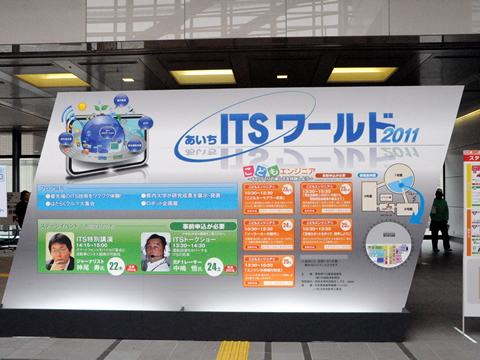
\includegraphics[autoebb,clip,height=4.0cm]{fig/ITSworld1.jpg}
	\quad
	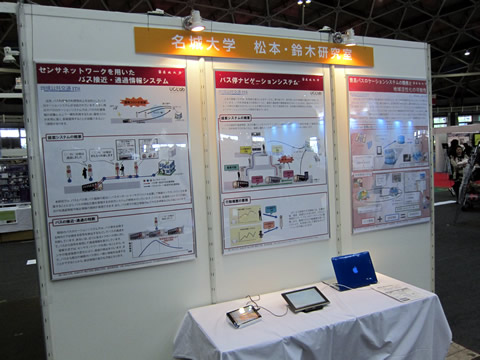
\includegraphics[autoebb,clip,height=4.0cm]{fig/ITSworld2.jpg}
	\caption{あいちITSワールド2011出展ブースの様子}
	\label{fig:ITSworld}
\end{figure}
\end{enumerate}

\endinput	% achievement.texの読み込み
\cleardoublepage

%--------------------------------------------------------------
% 付録
%--------------------------------------------------------------
\appendix
% 鈴木研究室 卒業論文付録テンプレート
% Version: 1.1
% Last Update: 2011/12/31 by Hidekazu Suzuki
% Contact to: hsuzuki@meijo-u.ac.jp
% Character code: UTF-8

\chapter{付録に掲載する内容例}\label{apdx:Example}

付録には本文の内容を補う情報,データなどを掲載するとよい.
例えば,以下のような内容が付録として適切である.

\begin{itemize}
\item プロトコル,シーケンス,パケットフォーマットなどの詳細情報
\item プログラムのソースコード
\item 実装の詳細な情報,インストール方法,実行方法など
\item 関連研究の詳細
\item 本文中に記載しなかった実験データおよび評価結果など
\item 研究の過程で得られた知見,修正したプログラムのバグなど
\end{itemize}


\section{ソースコードを掲載する方法}

ソースコードを掲載する場合は,下記の様に{\TeX}ファイルに直接コードを記述する方法と,外部のソースファイルを読み込む方法がある.
{\TeX}ファイルの可読性などを考慮すると,\subsecref{subsec:lstinputlisting}の読み込む方法を推奨する.


\subsection{{\TeX}ファイルに直接記述する場合}
\label{subsec:lstlisting}

ソースコードを{\TeX}ファイルに直接記述する場合は,\texttt{lstlisting}環境内にソースコードを記述する.
また,\texttt{lstlisting}環境のオプションとして,ソースコードのプログラミング言語\footnote{サポートされているプログラミング言語は,下記Webサイトを参照すること.\\\url{https://www.overleaf.com/learn/latex/Code_listing#Supported_languages}},キャプションおよび本文から参照するためのラベルを指定する.

\begin{code}
\begin{lstlisting}[language=プログラミング言語,caption=キャプション,label=src:ラベル]
ソースコードを記述
\end{lstlisting}
\end{code}%

素数を判定するPythonプログラムの記述例を\srcref{src:PrimeNumDescription}に示す.

\begin{lstlisting}[language=Python,caption=素数判定プログラム(直接記述の場合),label=src:PrimeNumDescription]
# 素数か否かを判定するプログラム

num = 29

# ユーザが入力する場合
#num = int(input("Enter a number: "))

# フラグ変数の定義
flag = False

if num == 1:
    print(num, "is not a prime number")
elif num > 1:
    # 約数のチェック
    for i in range(2, num):
        if (num % i) == 0:
            # 約数が見つかったらflagをTrueにする
            flag = True
            # ループを脱ける
            break

    # flagがTrueかチェック
    if flag:
        print(num, "is not a prime number")
    else:
        print(num, "is a prime number")
\end{lstlisting}


\subsection{ソースファイルを読み込む方法}
\label{subsec:lstinputlisting}

ソースファイルを{\TeX}ファイルに読み込んで掲載する場合は,\texttt{lstinputlisting}コマンドを用いる.
\texttt{lstinputlisting}のオプションは\subsecref{subsec:lstlisting}に示した\texttt{lstlisting}環境のオプションと同じである.

\begin{code}
\lstinputlisting[language=プログラミング言語,caption=キャプション,label=src:ラベル]{ソースファイルパス}
\end{code}%

素数を判定するPythonプログラムのソースファイル\texttt{src/primenum.py}の読み込み例を\srcref{src:PrimeNumFile}に示す.

\lstinputlisting[language=Python,caption=素数判定プログラム(ソースファイル読み込みの場合),label=src:PrimeNumFile]{src/primenum.py}



\chapter{使用しているパッケージと追加方法}\label{apdx:package}

本{\TeX}文章が採用しているスタイルファイル\texttt{UCLabThesis.sty}には,必要なスタイルファイルを利用するための記述がある.
各自の環境に必要なスタイルファイルがない場合は,下記の手順でスタイルを適用してほしい.
\begin{enumerate}
    \item インターネットから利用したいスタイルファイルを入手する.
    \item 各自のOverleaf環境にダウンロードしたスタイルファイルをアップロードする.
    \item \texttt{thesis.tex}で\texttt{UCLabThesis.sty}を読み込んでいる行の下に\verb|\usepackage{...}|を使ってスタイルファイルを適用する.
\end{enumerate}

\endinput	% appendix.texの読み込み

\end{document}
